\documentclass[usenames,dvipsnames]{beamer}
\usepackage{../../shared/styles/custom}
\usepackage{../../shared/styles/conventions}



\title{Decision Trees}
\date{\today}
\author{Nipun Batra and teaching staff}
\institute{IIT Gandhinagar}

% Define counter for pop quizzes
\newcounter{popquiz}
\setcounter{popquiz}{0}

\begin{document}
	\maketitle
	
	% Table of Contents
	\begin{frame}{Table of Contents}
		\tableofcontents[hideallsubsections]
	\end{frame}
	
	\section{Introduction and Motivation}
	
\begin{frame}{The need for interpretability}
	\begin{figure}
		\centering
		
\includegraphics[scale=0.32]{../assets/decision-trees/diagrams/interpretability}
		\label{fig:interpretability}
	\end{figure}
	
\end{frame}
	
	\renewcommand{\arraystretch}{0.85}
	\begin{frame}{Training Data}
	\begin{tabular}{lllll||l} \toprule
	\textbf{Day} & \textbf{Outlook}  & \textbf{Temp} & \textbf{Humidity} & \textbf{Windy}  & \textbf{Play} \\ \midrule
	D1  & Sunny    & Hot  & High     & Weak   & No   \\
	D2  & Sunny    & Hot  & High     & Strong & No   \\
	D3  & Overcast & Hot  & High     & Weak   & Yes  \\
	D4  & Rain     & Mild & High     & Weak   & Yes  \\
	D5  & Rain     & Cool & Normal   & Weak   & Yes  \\
	D6  & Rain     & Cool & Normal   & Strong & No   \\
	D7  & Overcast & Cool & Normal   & Strong & Yes  \\
	D8  & Sunny    & Mild & High     & Weak   & No   \\
	D9  & Sunny    & Cool & Normal   & Weak   & Yes  \\
	D10 & Rain     & Mild & Normal   & Weak   & Yes  \\
	D11 & Sunny    & Mild & Normal   & Strong & Yes  \\
	D12 & Overcast & Mild & High     & Strong & Yes  \\
	D13 & Overcast & Hot  & Normal   & Weak   & Yes  \\
	D14 & Rain     & Mild & High     & Strong & No  \\ \bottomrule
	\end{tabular}
\end{frame}

\begin{frame}{Learning a Complicated Neural Network}
\begin{figure}
	\centering
	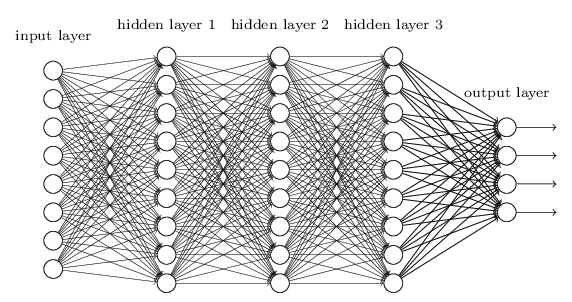
\includegraphics[width=1\linewidth]{../assets/decision-trees/diagrams/neural}
	
	\label{fig:neural}
\end{figure}
\end{frame}

\begin{frame}{Learnt Decision Tree}
\begin{tikzpicture}[
node/.style={%
	draw,
	rectangle,
},
]

\node [node] (A) {Outlook};
\path (A) ++(-150:\nodeDist) node [node] (B) {Humidity};
\path (A) ++(-90:\nodeDist/2) node [node, fill=green] (C) {Yes};
\path (A) ++(-30:\nodeDist) node [node] (D) {Wind};
\path (B) ++(-135:\nodeDist) node [node, fill=red] (E) {No};
\path (B) ++(-45:\nodeDist) node [node, fill=green] (F) {Yes};
\path (D) ++(-45:\nodeDist) node [node, fill=red] (G) {No};
\path (D) ++(-135:\nodeDist) node [node, fill=green] (H) {Yes};

\draw (A) -- (B) node [left,pos=0.25] {Sunny}(A);
\draw (A) -- (C) node [right,pos=0.8] {Overcast}(A);
\draw (A) -- (D) node [right,pos=0.5] {Rain}(A);
\draw (B) -- (E) node [left,pos=0.25] {High}(A);
\draw (B) -- (F) node [right,pos=0.25] {Normal}(C);
\draw (D) -- (G) node [right,pos=0.25] {Strong}(A);
\draw (D) -- (H) node [left,pos=0.25] {Weak}(A);
\end{tikzpicture}

\end{frame}

\begin{frame}{Medical Diagnosis using Decision Trees }
\begin{figure}
	\centering
	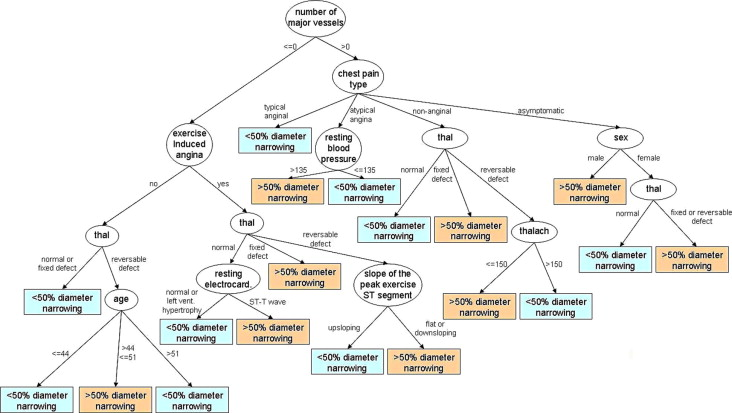
\includegraphics[width=1\linewidth]{../assets/decision-trees/diagrams/decision-medical}
	\caption{Source: Improving medical decision trees by combining relevant health-care criteria}
	\label{fig:decision-medical}
\end{figure}

\end{frame}


\begin{frame}{Leo Brieman}
\begin{figure}
	\centering
	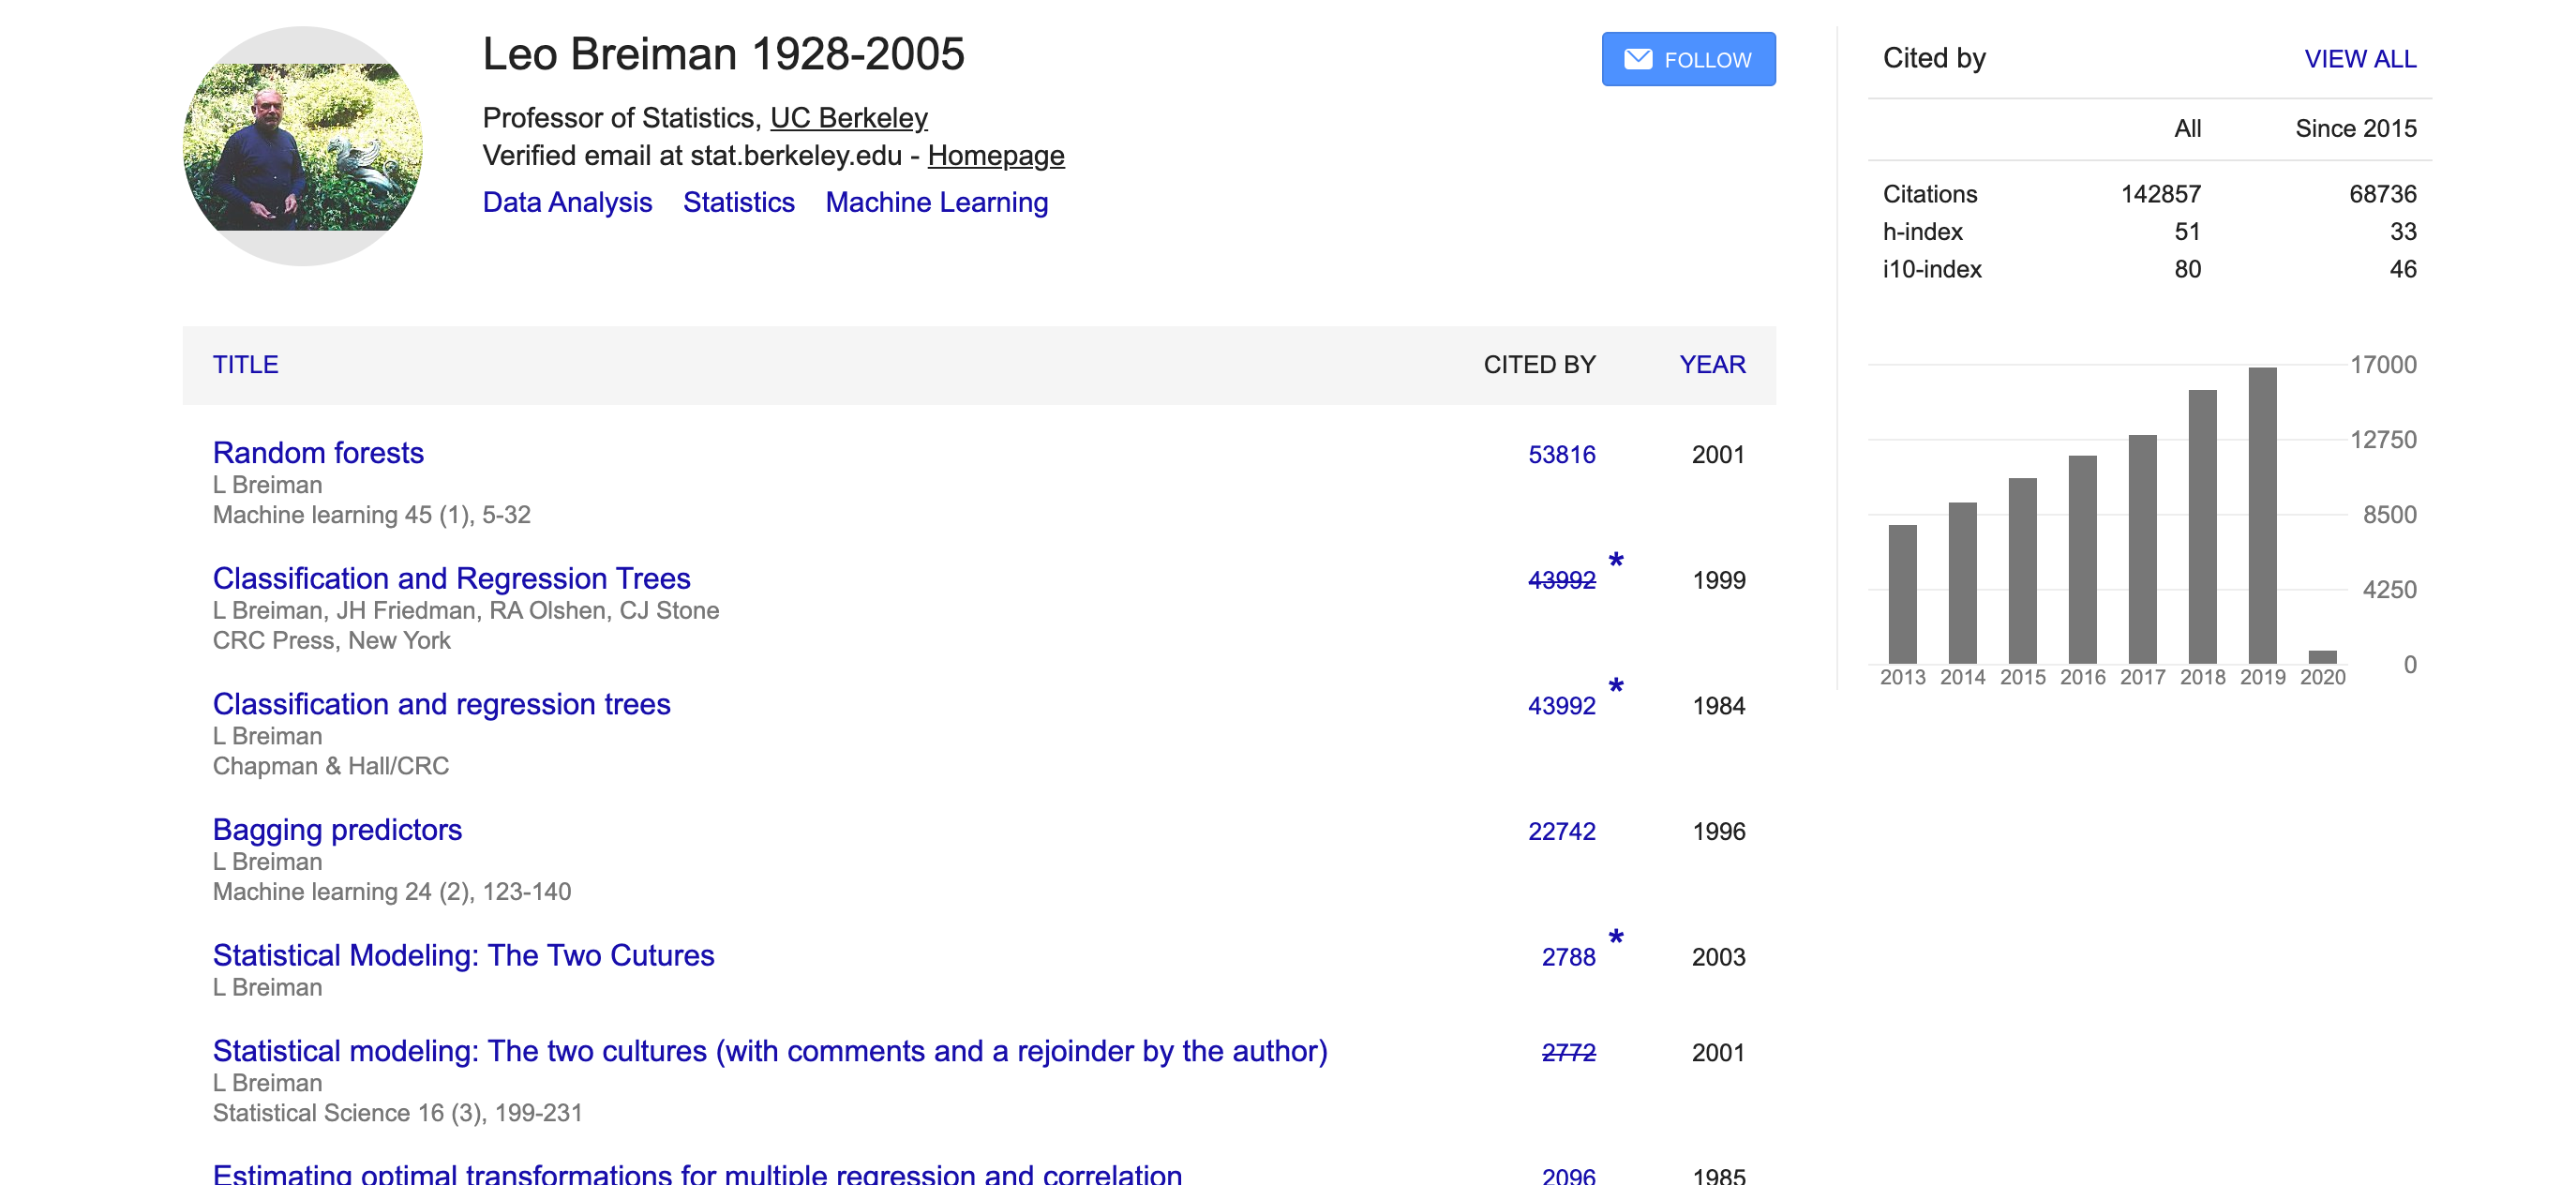
\includegraphics[width=1\linewidth]{../assets/decision-trees/diagrams/brieman}

	\label{fig:brieman}
\end{figure}

\end{frame}

\begin{frame}{Optimal Decision Tree}
\begin{figure}
	\centering
	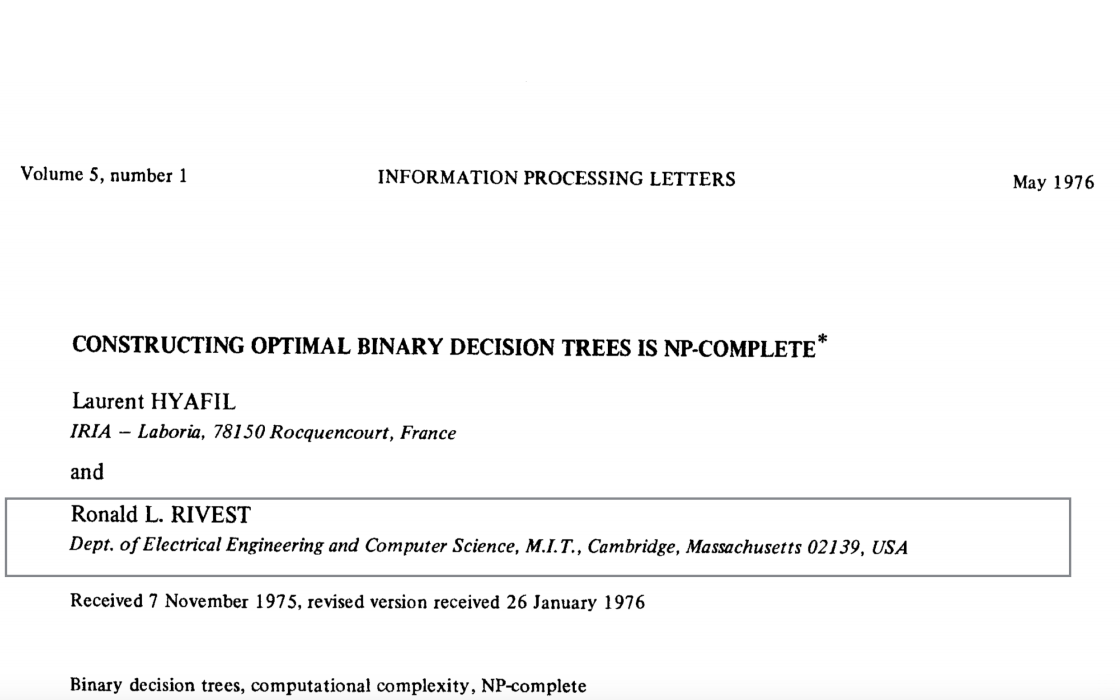
\includegraphics[width=1\linewidth]{../assets/decision-trees/diagrams/NP-hard}

	\label{fig:np-hard}
\end{figure}

\end{frame}

\begin{frame}{Pop Quiz \stepcounter{popquiz}\#\thepopquiz}
\begin{tcolorbox}[colback=blue!5!white,colframe=blue!75!black,title=Quick Question!]
Why is finding the optimal decision tree NP-hard?
\begin{enumerate}[A)]
\item The number of possible trees grows exponentially with features
\item We need to consider all possible splits at each node
\item The problem requires checking all subsets of training data
\item All of the above
\end{enumerate}
\pause
\textbf{Answer: D) All of the above} - The search space is exponentially large, making brute force optimization computationally intractable.
\end{tcolorbox}
\end{frame}

\begin{frame}{Greedy Algorithm}
Core idea: At each level, choose an attribute that gives
\textbf{biggest estimated} performance gain!

\begin{figure}
	\centering
	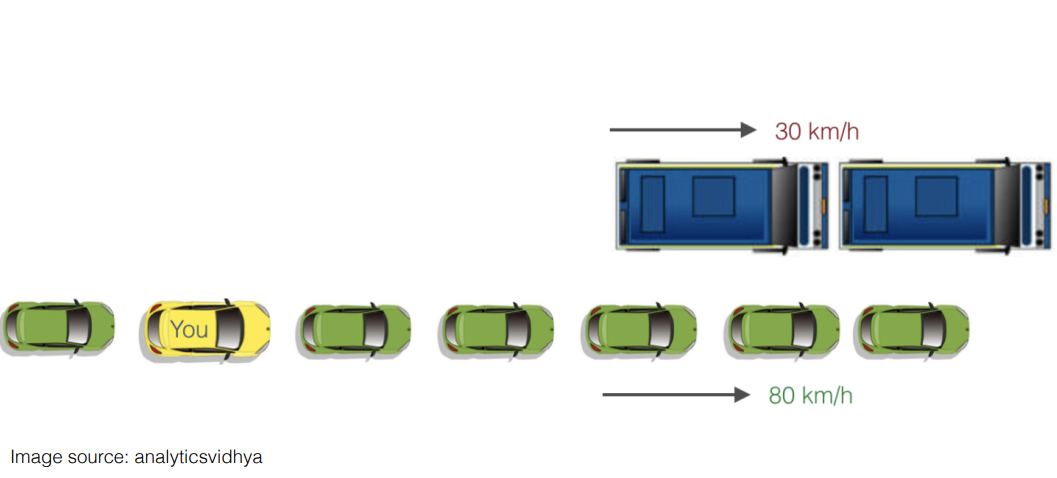
\includegraphics[width=0.8\linewidth]{../assets/decision-trees/diagrams/gredy}
	\caption{Greedy $\neq$ Optimal}
	\label{fig:gredy}
\end{figure}

\end{frame}

\begin{frame}{Towards biggest estimated performance gain}
\begin{columns}
\begin{column}{.7\textwidth}


\begin{scriptsize}


	\begin{tabular}{lllll||l} \toprule
	\textbf{Day} & \textbf{Outlook}  & \textbf{Temp} & \textbf{Humidity} & \textbf{Windy}  & \textbf{Play} \\ \midrule
	D1  & Sunny    & Hot  & High     & Weak   & No   \\
	D2  & Sunny    & Hot  & High     & Strong & No   \\
	D3  & Overcast & Hot  & High     & Weak   & Yes  \\
	D4  & Rain     & Mild & High     & Weak   & Yes  \\
	D5  & Rain     & Cool & Normal   & Weak   & Yes  \\
	D6  & Rain     & Cool & Normal   & Strong & No   \\
	D7  & Overcast & Cool & Normal   & Strong & Yes  \\
	D8  & Sunny    & Mild & High     & Weak   & No   \\
	D9  & Sunny    & Cool & Normal   & Weak   & Yes  \\
	D10 & Rain     & Mild & Normal   & Weak   & Yes  \\
	D11 & Sunny    & Mild & Normal   & Strong & Yes  \\
	D12 & Overcast & Mild & High     & Strong & Yes  \\
	D13 & Overcast & Hot  & Normal   & Weak   & Yes  \\
	D14 & Rain     & Mild & High     & Strong & No  \\ \bottomrule
\end{tabular}
\end{scriptsize}
\end{column}
\begin{column}{0.4\textwidth}
	\begin{scriptsize}
\begin{itemize}
	\pause \item For examples, we have 9 Yes, 5 No
	\pause \item Would it be trivial if we had 14 Yes or 14 No?
	\pause \item Yes!
	\pause \item Key insight: Problem is ``easier'' when there is less disagreement
	\pause 	\item Need some statistical measure of ``disagreement'' 
	\end{itemize}

\end{scriptsize}
\end{column}

\end{columns}

\end{frame}




%\begin{frame}
%\begin{forest}
%	for tree={grow'=south}
%	[Outlook
%	[Humidity, edge label={node[midway,fill=gray,font=\scriptsize]{Sunny}} []]
%	[Wind, edge label={node[midway,fill=white,font=\scriptsize]{Rain}} [] [] []]
%	[Yes, edge label={node[midway,fill=white,font=\scriptsize]{Overcast}}]
%	]
%\end{forest}
%\end{frame}

\begin{frame}{Entropy}
 Statistical measure to characterize the
(im)purity of examples

\pause $H(X) = -\sum_{i=1}^k p(x_i) \log_2 p(x_i)$

\begin{figure}[htp]
    \centering
    \begin{notebookbox}{https://nipunbatra.github.io/ml-teaching/notebooks/entropy.html}
      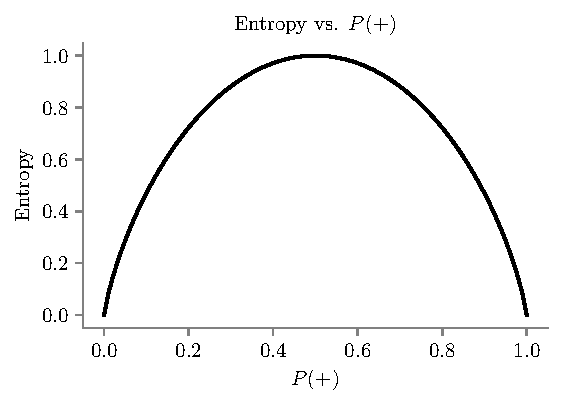
\includegraphics[scale=0.6]{../assets/decision-trees/figures/entropy.pdf}
    \end{notebookbox}
  \end{figure}

\end{frame}
	
\begin{frame}{Towards biggest estimated performance gain}
\begin{columns}
	\begin{column}{.7\textwidth}
		
		
		\begin{scriptsize}
			

			\begin{tabular}{lllll||l} \toprule
				\textbf{Day} & \textbf{Outlook}  & \textbf{Temp} & \textbf{Humidity} & \textbf{Windy}  & \textbf{Play} \\ \midrule
				D1  & Sunny    & Hot  & High     & Weak   & No   \\
				D2  & Sunny    & Hot  & High     & Strong & No   \\
				D3  & Overcast & Hot  & High     & Weak   & Yes  \\
				D4  & Rain     & Mild & High     & Weak   & Yes  \\
				D5  & Rain     & Cool & Normal   & Weak   & Yes  \\
				D6  & Rain     & Cool & Normal   & Strong & No   \\
				D7  & Overcast & Cool & Normal   & Strong & Yes  \\
				D8  & Sunny    & Mild & High     & Weak   & No   \\
				D9  & Sunny    & Cool & Normal   & Weak   & Yes  \\
				D10 & Rain     & Mild & Normal   & Weak   & Yes  \\
				D11 & Sunny    & Mild & Normal   & Strong & Yes  \\
				D12 & Overcast & Mild & High     & Strong & Yes  \\
				D13 & Overcast & Hot  & Normal   & Weak   & Yes  \\
				D14 & Rain     & Mild & High     & Strong & No  \\ \bottomrule
			\end{tabular}
		\end{scriptsize}
	\end{column}
	\begin{column}{0.4\textwidth}
		\begin{scriptsize}
			\begin{itemize}
				\pause \item Can we use Outlook as the root node?
				\pause 	\item When Outlook is overcast, we always Play and thus no ``disagreement'' 
			\end{itemize}
			
		\end{scriptsize}
	\end{column}
	
\end{columns}

\end{frame}
	
\begin{frame}{Information Gain}
 Reduction in entropy
by partitioning examples (S) on attribute A
$$
\operatorname{Gain}(S, A) \equiv \text{Entropy}(S)-\sum_{v \in \text{Values}(A)} \frac{|S_{v}|}{|S|} \text{Entropy}(S_{v})
$$
\end{frame}

\begin{frame}{Pop Quiz \stepcounter{popquiz}\#\thepopquiz}
\begin{tcolorbox}[colback=blue!5!white,colframe=blue!75!black,title=Quick Question!]
What does entropy measure in the context of decision trees?
\begin{enumerate}[A)]
\item The depth of the tree
\item The impurity or "disagreement" in a set of examples
\item The number of features in the dataset
\item The accuracy of the tree
\end{enumerate}
\pause
\textbf{Answer: B) The impurity or "disagreement" in a set of examples} - Higher entropy means more mixed classes, lower entropy means more pure subsets.
\end{tcolorbox}
\end{frame}


\begin{frame}{ID3 (Examples, Target Attribute, Attributes)}
\begin{itemize}[<+->]
	\item Create a root node for tree
	\item If all examples are +/-, return root with label = +/-
	\item  If attributes = empty, return root with most common value of
	Target Attribute in Examples
	\item Begin
	\begin{itemize}[<+->]
		\item A $\leftarrow$ attribute from Attributes which best classifies
		Examples
		\item 	Root $\leftarrow$ A
		\item  For each value (v) of A
		\begin{itemize}[<+->]
			\item Add new tree branch : A = v
			\item  Examples\textsubscript{v}: subset of examples that A = v
			\item If Examples\textsubscript{v}is empty: add leaf with label = most
			common value of Target Attribute
			\item Else: ID3 (Examples\textsubscript{v}, Target attribute, Attributes - {A})
		\end{itemize}
	\end{itemize}


\end{itemize}
\end{frame}

\begin{frame}{Learnt Decision Tree}
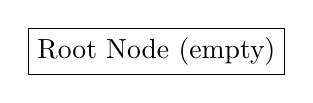
\begin{tikzpicture}[
node/.style={%
	draw,
	rectangle,
},
]

\node [node] (A) {Root Node (empty)};

\end{tikzpicture}

\end{frame}

	\begin{frame}{Training Data}
\begin{tabular}{lllll||l} \toprule
	\textbf{Day} & \textbf{Outlook}  & \textbf{Temp} & \textbf{Humidity} & \textbf{Windy}  & \textbf{Play} \\ \midrule
	D1  & Sunny    & Hot  & High     & Weak   & No   \\
	D2  & Sunny    & Hot  & High     & Strong & No   \\
	D3  & Overcast & Hot  & High     & Weak   & Yes  \\
	D4  & Rain     & Mild & High     & Weak   & Yes  \\
	D5  & Rain     & Cool & Normal   & Weak   & Yes  \\
	D6  & Rain     & Cool & Normal   & Strong & No   \\
	D7  & Overcast & Cool & Normal   & Strong & Yes  \\
	D8  & Sunny    & Mild & High     & Weak   & No   \\
	D9  & Sunny    & Cool & Normal   & Weak   & Yes  \\
	D10 & Rain     & Mild & Normal   & Weak   & Yes  \\
	D11 & Sunny    & Mild & Normal   & Strong & Yes  \\
	D12 & Overcast & Mild & High     & Strong & Yes  \\
	D13 & Overcast & Hot  & Normal   & Weak   & Yes  \\
	D14 & Rain     & Mild & High     & Strong & No  \\ \bottomrule
\end{tabular}
\end{frame}


\begin{frame}{Entropy calculated}
We have 14 examples in $S$: 5 No, 9 Yes

$$\Entropy(S) = -p_{\text{No}} \log_2 p_{\text{No}} - p_{\text{Yes}} \log_2 p_{\text{Yes}}$$
$$
= -\frac{5}{14} \log_2\left(\frac{5}{14}\right) - \frac{9}{14} \log_2\left(\frac{9}{14}\right) = 0.940
$$
\end{frame}

\begin{frame}{Information Gain for Outlook}
\begin{tabular}{l|l} \toprule
\textbf{Outlook} & \textbf{Play} \\ \midrule
Sunny    & No   \\
Sunny    & No   \\
Overcast & Yes  \\
Rain     & Yes  \\
Rain     & Yes  \\
Rain     & No   \\
Overcast & Yes  \\
Sunny    & No   \\
Sunny    & Yes  \\
Rain     & Yes  \\
Sunny    & Yes  \\
Overcast & Yes  \\
Overcast & Yes  \\
Rain     & No  \\ \bottomrule
\end{tabular}
\end{frame}

\begin{frame}{Information Gain for Outlook}
\begin{columns}


\begin{column}{.32\textwidth}
	\begin{table}
\begin{tabular}{l|l} \toprule
	\textbf{Outlook} & \textbf{Play} \\ \midrule
	Sunny    & No   \\
	Sunny    & No   \\
	Sunny    & No   \\
	Sunny    & Yes  \\
	Sunny    & Yes  \\

\bottomrule
\end{tabular}
We have 2 Yes, 3 No
$\Entropy = -\frac{3}{5} \log_2\left(\frac{3}{5}\right) - \frac{2}{5} \log_2\left(\frac{2}{5}\right) = 0.971$
\end{table}
\end{column}

\pause \begin{column}{.32\textwidth}
	\begin{table}


\begin{tabular}{l|l} \toprule
	\textbf{Outlook} & \textbf{Play} \\ \midrule

	Overcast & Yes  \\
	Overcast & Yes  \\
	Overcast & Yes  \\
	Overcast & Yes  \\ \bottomrule

\end{tabular}
We have 4 Yes, 0 No
$\Entropy = 0$ (pure subset)


	\end{table}


\end{column}


\pause \begin{column}{.32\textwidth}
	\begin{table}
\begin{tabular}{l|l} \toprule
	\textbf{Outlook} & \textbf{Play} \\ \midrule
	Rain     & Yes  \\
	Rain     & Yes  \\
	Rain     & No   \\
	Rain     & Yes  \\
	Rain     & No  \\ \bottomrule
\end{tabular}
We have 3 Yes, 2 No
$\Entropy = -\frac{3}{5} \log_2\left(\frac{3}{5}\right) - \frac{2}{5} \log_2\left(\frac{2}{5}\right) = 0.971$
\end{table}
\end{column}
\end{columns}
\end{frame}

\begin{frame}{Information Gain}
$$
\operatorname{Gain}(S, \text{Outlook}) = \text{Entropy}(S)-\sum_{v \in \{\text{Rain, Sunny, Overcast}\}} \frac{|S_{v}|}{|S|} \text{Entropy}(S_{v}) 
$$

\[
\Gain(S, \text{Outlook}) = \Entropy(S) - \frac{5}{14} \Entropy(S_{\text{Sunny}}) - \frac{4}{14} \Entropy(S_{\text{Overcast}}) - \frac{5}{14} \Entropy(S_{\text{Rain}})
\]
\[
= 0.940 - \frac{5}{14} \times 0.971 - \frac{4}{14} \times 0 - \frac{5}{14} \times 0.971 = 0.940 - 0.347 - 0 - 0.347 = 0.246
\]

\end{frame}

\begin{frame}{Information Gain}


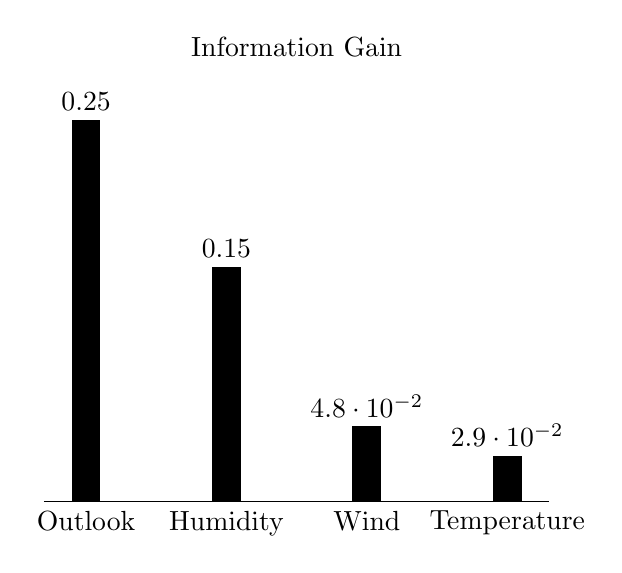
\begin{tikzpicture}
\begin{axis}[
symbolic x coords={Outlook,Humidity,Wind,Temperature},
xtick=data,xtick pos=left, width=8cm,
ytick pos=left,axis x line*=bottom,nodes near coords,hide y axis,title=Information Gain, ymin=0.0]
\addplot[ybar,fill=black] coordinates {
	(Outlook,0.246)
	(Humidity,0.151)
	(Wind,0.048)
	(Temperature,0.029)
};
\end{axis}
\end{tikzpicture}


\end{frame}

\begin{frame}{Learnt Decision Tree}
\begin{tikzpicture}[
node/.style={%
	draw,
	rectangle,
},
]

\node [node] (A) {Outlook};
\path (A) ++(-150:\nodeDist) node [node] (B) {?};
\path (A) ++(-90:\nodeDist/2) node [node, fill=green] (C) {Yes};
\path (A) ++(-30:\nodeDist) node [node] (D) {?};


\draw (A) -- (B) node [left,pos=0.25] {Sunny}(A);
\draw (A) -- (C) node [right,pos=0.8] {Overcast}(A);
\draw (A) -- (D) node [right,pos=0.5] {Rain}(A);

\end{tikzpicture}

\end{frame}

	\begin{frame}{Calling ID3 on Outlook=Sunny}
\begin{tabular}{llll||l} \toprule
	\textbf{Day} & \textbf{Temp} & \textbf{Humidity} & \textbf{Windy}  & \textbf{Play} \\ \midrule
	D1    & Hot  & High     & Weak   & No   \\
	D2     & Hot  & High     & Strong & No   \\
	D8     & Mild & High     & Weak   & No   \\
	D9    & Cool & Normal   & Weak   & Yes  \\
	D11    & Mild & Normal   & Strong & Yes  \\ \bottomrule
\end{tabular}

\begin{itemize}
	\pause \item Gain($S_{\text{Outlook=Sunny}}$, Temp) = Entropy(2 Yes, 3 No) - (2/5)*Entropy(0 Yes, 2 No) -(2/5)*Entropy(1 Yes, 1 No) - (1/5)*Entropy(1 Yes, 0 No) 
	\pause \item Gain($S_{\text{Outlook=Sunny}}$, Humidity) = Entropy(2 Yes, 3 No) - (2/5)*Entropy(2 Yes, 0 No) -(3/5)*Entropy(0 Yes, 3 No) $\implies$ \textbf{maximum possible for the set}
	\pause \item Gain($S_{\text{Outlook=Sunny}}$, Windy) = Entropy(2 Yes, 3 No) - (3/5)*Entropy(1 Yes, 2 No) -(2/5)*Entropy(1 Yes, 1 No) 
\end{itemize}
\end{frame}

\begin{frame}{Learnt Decision Tree}
\begin{tikzpicture}[
node/.style={%
	draw,
	rectangle,
},
]

\node [node] (A) {Outlook};
\path (A) ++(-150:\nodeDist) node [node] (B) {Humidity};
\path (A) ++(-90:\nodeDist/2) node [node, fill=green] (C) {Yes};
\path (A) ++(-30:\nodeDist) node [node] (D) {?};
\path (B) ++(-135:\nodeDist) node [node, fill=red] (E) {No};
\path (B) ++(-45:\nodeDist) node [node, fill=green] (F) {Yes};
;

\draw (A) -- (B) node [left,pos=0.25] {Sunny}(A);
\draw (A) -- (C) node [right,pos=0.8] {Overcast}(A);
\draw (A) -- (D) node [right,pos=0.5] {Rain}(A);
\draw (B) -- (E) node [left,pos=0.25] {High}(A);
\draw (B) -- (F) node [right,pos=0.25] {Normal}(C);

\end{tikzpicture}

\end{frame}


	\begin{frame}{Calling ID3 on (Outlook=Rain)}
\begin{tabular}{llll||l} \toprule
	\textbf{Day}  & \textbf{Temp} & \textbf{Humidity} & \textbf{Windy}  & \textbf{Play} \\ \midrule
	D4    & Mild & High     & Weak   & Yes  \\
	D5     & Cool & Normal   & Weak   & Yes  \\
	D6      & Cool & Normal   & Strong & No   \\
	D10     & Mild & Normal   & Weak   & Yes  \\
	D14      & Mild & High     & Strong & No  \\ \bottomrule
\end{tabular}
\begin{itemize}
	\item The attribute Windy gives the highest information gain
\end{itemize}
\end{frame}

\begin{frame}{Learnt Decision Tree}
\begin{tikzpicture}[
node/.style={%
	draw,
	rectangle,
},
]

\node [node] (A) {Outlook};
\path (A) ++(-150:\nodeDist) node [node] (B) {Humidity};
\path (A) ++(-90:\nodeDist/2) node [node, fill=green] (C) {Yes};
\path (A) ++(-30:\nodeDist) node [node] (D) {Wind};
\path (B) ++(-135:\nodeDist) node [node, fill=red] (E) {No};
\path (B) ++(-45:\nodeDist) node [node, fill=green] (F) {Yes};
\path (D) ++(-45:\nodeDist) node [node, fill=red] (G) {No};
\path (D) ++(-135:\nodeDist) node [node, fill=green] (H) {Yes};

\draw (A) -- (B) node [left,pos=0.25] {Sunny}(A);
\draw (A) -- (C) node [right,pos=0.8] {Overcast}(A);
\draw (A) -- (D) node [right,pos=0.5] {Rain}(A);
\draw (B) -- (E) node [left,pos=0.25] {High}(A);
\draw (B) -- (F) node [right,pos=0.25] {Normal}(C);
\draw (D) -- (G) node [right,pos=0.25] {Strong}(A);
\draw (D) -- (H) node [left,pos=0.25] {Weak}(A);
\end{tikzpicture}

\end{frame}

\begin{frame}{Prediction for Decision Tree}
Just walk down the tree!

\begin{tikzpicture}[
node/.style={%
	draw,
	rectangle,
},
]

\node [node] (A) {Outlook};
\path (A) ++(-150:\nodeDist) node [node] (B) {Humidity};
\path (A) ++(-90:\nodeDist/2) node [node, fill=green] (C) {Yes};
\path (A) ++(-30:\nodeDist) node [node] (D) {Wind};
\path (B) ++(-135:\nodeDist) node [node, fill=red] (E) {No};
\path (B) ++(-45:\nodeDist) node [node, fill=green] (F) {Yes};
\path (D) ++(-45:\nodeDist) node [node, fill=red] (G) {No};
\path (D) ++(-135:\nodeDist) node [node, fill=green] (H) {Yes};

\draw (A) -- (B) node [left,pos=0.25] {Sunny}(A);
\draw (A) -- (C) node [right,pos=0.8] {Overcast}(A);
\draw (A) -- (D) node [right,pos=0.5] {Rain}(A);
\draw (B) -- (E) node [left,pos=0.25] {High}(A);
\draw (B) -- (F) node [right,pos=0.25] {Normal}(C);
\draw (D) -- (G) node [right,pos=0.25] {Strong}(A);
\draw (D) -- (H) node [left,pos=0.25] {Weak}(A);
\end{tikzpicture}

\pause Prediction for $<$High Humidity, Strong Wind, Sunny Outlook, Hot Temp$>$ is ? \\
\pause  No
\end{frame}

\begin{frame}{Limiting Depth of Tree}
Assuming if you were only allowed depth-$1$ trees, how would it look for the current dataset? \\

\pause Apply the same rules, except when depth limit is reached, the leaf node is assigned the most common occurring value in that path.

\pause What is depth-$0$ tree (no decision) for the examples? \\
\pause Always predicting Yes

\pause What is depth-$1$ tree (no decision) for the examples? \\
\pause \begin{tikzpicture}[
node/.style={%
	draw,
	rectangle,
},
]

\node [node] (A) {Outlook};
\path (A) ++(-150:\nodeDist) node [node, fill=red] (B) {No};
\path (A) ++(-90:\nodeDist/2) node [node, fill=green] (C) {Yes};
\path (A) ++(-30:\nodeDist) node [node, fill=green] (D) {Yes};


\draw (A) -- (B) node [left,pos=0.25] {Sunny}(A);
\draw (A) -- (C) node [right,pos=0.8] {Overcast}(A);
\draw (A) -- (D) node [right,pos=0.5] {Rain}(A);

\end{tikzpicture}

\end{frame}

\begin{frame}{Pop Quiz \stepcounter{popquiz}\#\thepopquiz}
\begin{tcolorbox}[colback=blue!5!white,colframe=blue!75!black,title=Quick Question!]
In the tennis dataset, why did "Outlook" have the highest information gain?
\begin{enumerate}[A)]
\item It was the first feature in the dataset
\item When Outlook=Overcast, all examples have Play=Yes (pure subset)
\item It has the most possible values
\item It was chosen randomly
\end{enumerate}
\pause
\textbf{Answer: B) When Outlook=Overcast, all examples have Play=Yes} - This creates a pure subset with entropy=0, maximizing information gain.
\end{tcolorbox}
\end{frame}

\section{Discrete Input, Real Output}

\begin{frame}{Modified Dataset}
\begin{table}[]
	\begin{tabular}{@{}llllll@{}}
		\toprule
		\textbf{Day} & \textbf{Outlook} & \textbf{Temp} & \textbf{Humidity} & \textbf{Wind} & \textbf{Minutes Played} \\ \midrule
		D1           & Sunny            & Hot           & High              & Weak          & 20                      \\
		D2           & Sunny            & Hot           & High              & Strong        & 24                      \\
		D3           & Overcast         & Hot           & High              & Weak          & 40                      \\
		D4           & Rain             & Mild          & High              & Weak          & 50                      \\
		D5           & Rain             & Cool          & Normal            & Weak          & 60                      \\
		D6           & Rain             & Cool          & Normal            & Strong        & 10                      \\
		D7           & Overcast         & Cool          & Normal            & Strong        & 4                       \\
		D8           & Sunny            & Mild          & High              & Weak          & 10                      \\
		D9           & Sunny            & Cool          & Normal            & Weak          & 60                      \\
		D10          & Rain             & Mild          & Normal            & Weak          & 40                      \\
		D11          & Sunny            & Mild          & High              & Strong        & 45                      \\
		D12          & Overcast         & Mild          & High              & Strong        & 40                      \\
		D13          & Overcast         & Hot           & Normal            & Weak          & 35                      \\
		D14          & Rain             & Mild          & High              & Strong        & 20                      \\ \bottomrule
	\end{tabular}
\end{table}
\end{frame}

\begin{frame}{Measure of Impurity for Regression?}
\begin{itemize}
	\item \pause Any guesses?
	\item \pause Mean Squared Error
	\item \pause $\MSE(S) = 311.34$
	\item \pause What about splitting criterion for regression?
	\item \pause \textbf{MSE Reduction} (not Information Gain!)
	\item \pause MSE Reduction = $\MSE(S) - \sum_{v} \frac{|S_v|}{|S|} \MSE(S_v)$
\end{itemize}

\end{frame}

\begin{frame}{Gain by splitting on Wind}
\begin{columns}

\begin{column}{.5\textwidth}
	\begin{scriptsize}

\begin{table}[]
	\begin{tabular}{@{}ll@{}}
		\toprule
		\textbf{Wind} & \textbf{Minutes Played} \\ \midrule
		Weak          & 20                      \\
		Strong        & 24                      \\
		Weak          & 40                      \\
		Weak          & 50                      \\
		Weak          & 60                      \\
		Strong        & 10                      \\
		Strong        & 4                       \\
		Weak          & 10                      \\
		Weak          & 60                      \\
		Weak          & 40                      \\
		Strong        & 45                      \\
		Strong        & 40                      \\
		Weak          & 35                      \\
		Strong        & 20                      \\ \bottomrule
	\end{tabular}
\caption{MSE(S)=311.34}
\end{table}
	\end{scriptsize}
\end{column}
\begin{column}{.5\textwidth}
	\begin{tiny}
\vspace{-5pt}		
\begin{table}[]
	\begin{tabular}{@{}ll@{}}
		\toprule
		\textbf{Wind} & \textbf{Minutes Played} \\ \midrule
		Weak          & 20                      \\
		Weak          & 40                      \\
		Weak          & 50                      \\
		Weak          & 60                      \\
		Weak          & 10                      \\
		Weak          & 60                      \\
		Weak          & 40                      \\
		Weak          & 35                      \\ \bottomrule
	\end{tabular}
\caption{$\MSE(S_{\text{Wind=Weak}}) = 277$, Weight = $\frac{8}{14}$}
\end{table}
\vspace{-25pt}
	\end{tiny}

	\begin{tiny}
	
	\begin{table}[]
		\begin{tabular}{@{}ll@{}}
			\toprule
			\textbf{Wind} & \textbf{Minutes Played} \\ \midrule

			Strong        & 24                      \\
			Strong        & 10                      \\
			Strong        & 4                       \\
			Strong        & 45                      \\
			Strong        & 40                      \\
			Strong        & 20                      \\ \bottomrule
		\end{tabular}
\caption{$\MSE(S_{\text{Wind=Strong}}) = 218$, Weight = $\frac{6}{14}$}
	\end{table}
\end{tiny}

\end{column}
\end{columns}
\end{frame}

\begin{frame}{MSE Reduction Calculation}
\textbf{Correct calculation for Wind split:}
\[
\text{MSE Reduction} = \MSE(S) - \text{Weighted Average MSE}
\]
\[
= 311.34 - \left[\frac{8}{14} \times 277 + \frac{6}{14} \times 218\right] = 311.34 - [158.857 + 93.429] = 311.34 - 252.286 = \mathbf{59.05}
\]

\textbf{Key insight:} MSE Reduction $> 0$ means the split improves our model!

\textbf{For regression:} Use MSE Reduction, NOT Information Gain!
\end{frame}

\begin{frame}{Pop Quiz \stepcounter{popquiz}\#\thepopquiz}
\begin{tcolorbox}[colback=blue!5!white,colframe=blue!75!black,title=Quick Question!]
For regression trees, what criterion do we use instead of Information Gain?
\begin{enumerate}[A)]
\item Information Gain
\item Gini Impurity
\item Mean Squared Error (MSE) Reduction
\item Accuracy
\end{enumerate}
\pause
\textbf{Answer: C) Mean Squared Error (MSE) Reduction} - For regression, we minimize MSE instead of maximizing information gain.
\end{tcolorbox}
\end{frame}

\begin{frame}{MSE Reduction for Regression Trees}

	\begin{figure}[htp]
		\centering
		\begin{notebookbox}{https://nipunbatra.github.io/ml-teaching/notebooks/decision-tree-real-output.html}
		  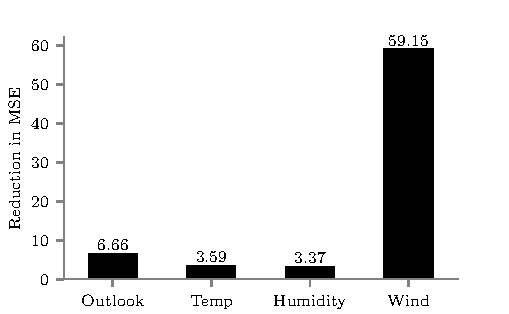
\includegraphics[width=\linewidth]{../assets/decision-trees/figures/discrete-input-real-output-level-1.pdf}
		\end{notebookbox}
	  \end{figure}

\end{frame}

\begin{frame}{Learnt Tree}
\begin{figure}
	\centering
	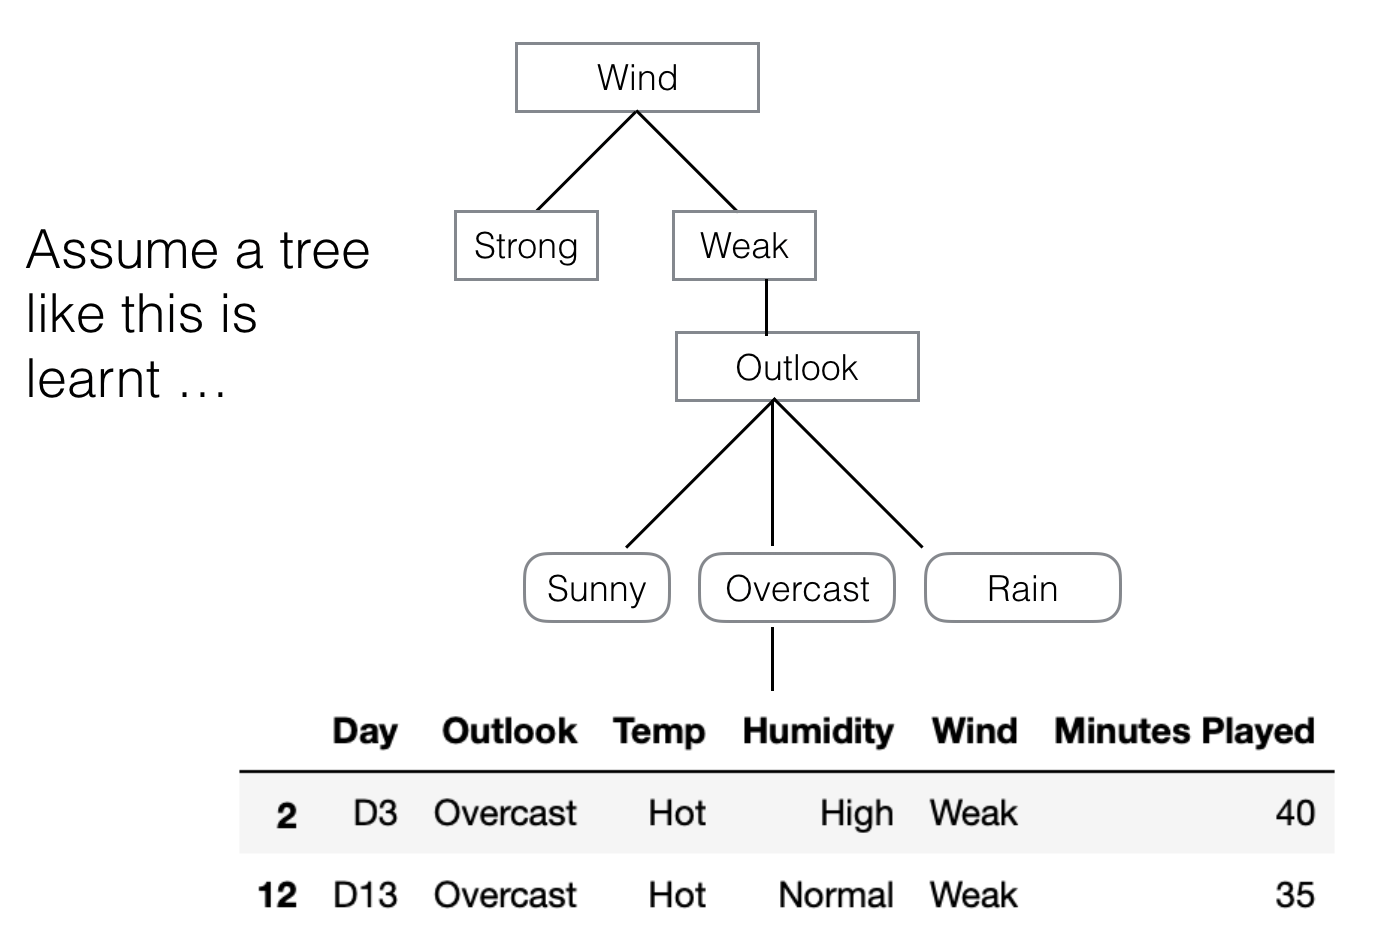
\includegraphics[width=1\linewidth]{../assets/decision-trees/diagrams/tree}

	\label{fig:tree}
\end{figure}

\end{frame}

\begin{frame}{Learnt Tree}
\begin{figure}
	\centering
	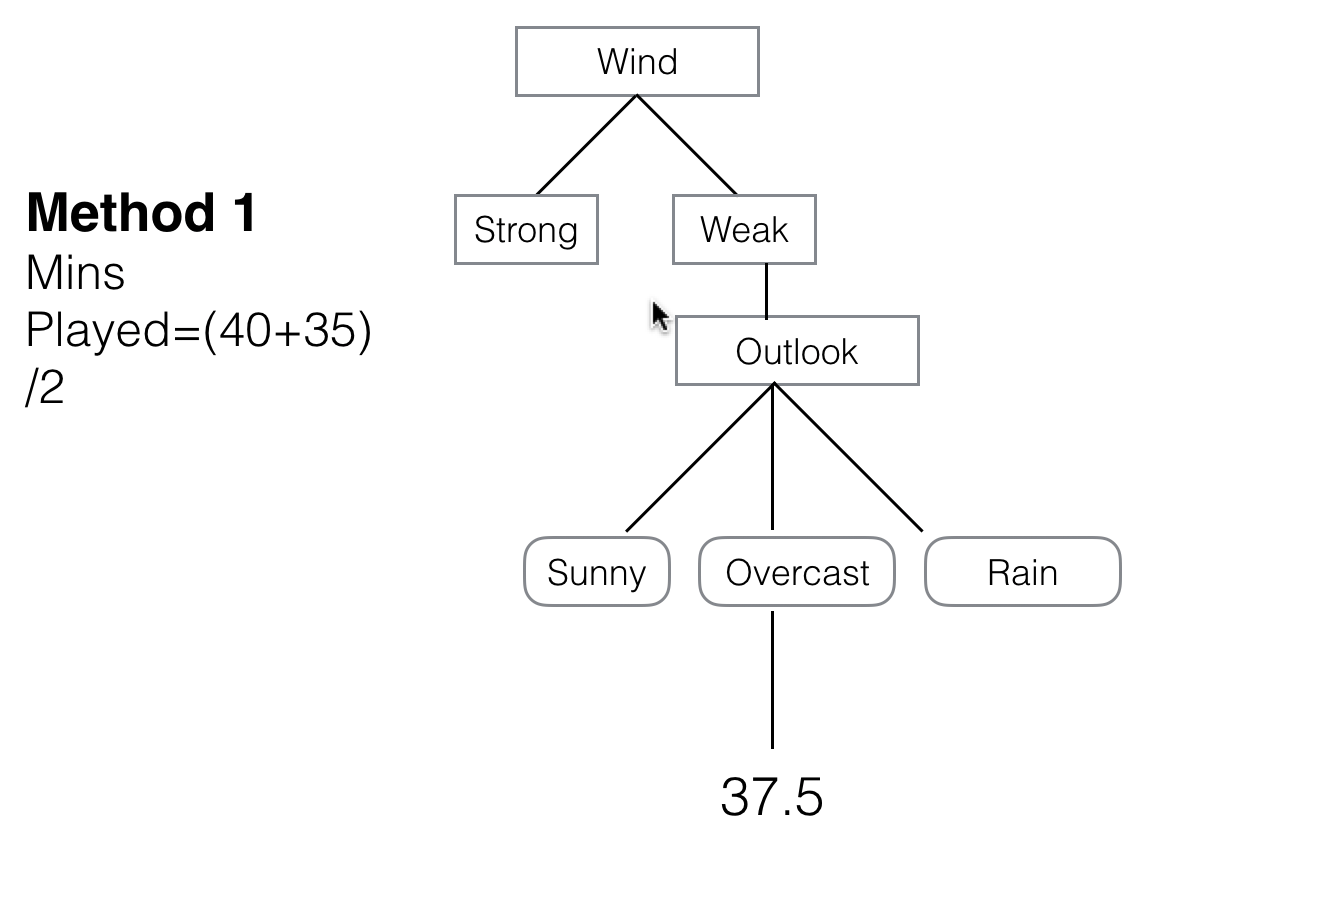
\includegraphics[width=1\linewidth]{../assets/decision-trees/diagrams/tree2}

	\label{fig:tree}
\end{figure}

\end{frame}

\section{Real Input Discrete Output}


\begin{frame}{Finding splits}
\begin{table}[]
	\begin{tabular}{@{}lrr@{}}
		\toprule
		\textbf{Day} & \textbf{Temperature} & \textbf{PlayTennis} \\ \midrule
		D1           & 40                   & No                  \\
		D2           & 48                   & No                  \\
		D3           & 60                   & Yes                 \\
		D4           & 72                   & Yes                 \\
		D5           & 80                   & Yes                 \\
		D6           & 90                   & No                  \\ \bottomrule
	\end{tabular}
\end{table}
\begin{itemize}[<+->]
	\item How do you find splits?
	\item Sort by attribute
	\item Find potential split points (midpoints). 
	\item For the above example, we have 5 potential splits: 44, 54, 66, 76, 85
	\item Calculate the weighted impurity for each split
	\item Choose the split with the lowest impurity
\end{itemize}
\end{frame}

\begin{frame}{Finding splits}
	\begin{table}[]
		\begin{tabular}{@{}lrr@{}}
			\toprule
			\textbf{Day} & \textbf{Temperature} & \textbf{PlayTennis} \\ \midrule
			D1           & 40                   & No                  \\
			D2           & 48                   & No                  \\
			D3           & 60                   & Yes                 \\
			D4           & 72                   & Yes                 \\
			D5           & 80                   & Yes                 \\
			D6           & 90                   & No                  \\ \bottomrule
		\end{tabular}
	\end{table}
	\begin{itemize}
		\item Consider split at 44
		\item LHS has 1 No and 0 Yes; RHS has 3 Yes and 2 No
		\item Entropy for LHS = 0, Entropy for RHS = 0.971
		\item Weighted Entropy = 0.971*5/6 = 0.808
	\end{itemize}
	\end{frame}

	\begin{frame}{Finding splits}
		\begin{table}[]
			\begin{tabular}{@{}lrr@{}}
				\toprule
				\textbf{Day} & \textbf{Temperature} & \textbf{PlayTennis} \\ \midrule
				D1           & 40                   & No                  \\
				D2           & 48                   & No                  \\
				D3           & 60                   & Yes                 \\
				D4           & 72                   & Yes                 \\
				D5           & 80                   & Yes                 \\
				D6           & 90                   & No                  \\ \bottomrule
			\end{tabular}
		\end{table}
		\begin{itemize}
			\item Consider split at 54
			\item LHS has 2 No and 0 Yes; RHS has 3 Yes and 1 No
			\item Entropy for LHS = 0, Entropy for RHS = 0.811
			\item Weighted Entropy = 0.811*4/6 = 0.541
		\end{itemize}
		\end{frame}

		\begin{frame}{Finding splits}
			\begin{table}[]
				\begin{tabular}{@{}lrr@{}}
					\toprule
					\textbf{Day} & \textbf{Temperature} & \textbf{PlayTennis} \\ \midrule
					D1           & 40                   & No                  \\
					D2           & 48                   & No                  \\
					D3           & 60                   & Yes                 \\
					D4           & 72                   & Yes                 \\
					D5           & 80                   & Yes                 \\
					D6           & 90                   & No                  \\ \bottomrule
				\end{tabular}
			\end{table}
			\begin{itemize}
				\item Consider split at 66
				\item LHS has 2 No and 1 Yes; RHS has 2 Yes and 1 No
				\item Entropy for LHS = 0.918, Entropy for RHS = 0.918
				\item Weighted Entropy = 0.918*3/6 + 0.918*3/6 = 0.918
			\end{itemize}
			\end{frame}


		\begin{frame}{Finding splits}
			\begin{table}[]
				\begin{tabular}{@{}lrr@{}}
					\toprule
					\textbf{Day} & \textbf{Temperature} & \textbf{PlayTennis} \\ \midrule
					D1           & 40                   & No                  \\
					D2           & 48                   & No                  \\
					D3           & 60                   & Yes                 \\
					D4           & 72                   & Yes                 \\
					D5           & 80                   & Yes                 \\
					D6           & 90                   & No                  \\ \bottomrule
				\end{tabular}
			\end{table}
			\begin{itemize}
				\item Consider split at 76
				\item LHS has 2 No and 2 Yes; RHS has 1 Yes and 1 No
				\item Entropy for LHS = 1, Entropy for RHS = 1
				\item Weighted Entropy = 1*4/6 + 1*2/6 = 1
			\end{itemize}
			\end{frame}

			\begin{frame}{Finding splits}
				\begin{table}[]
					\begin{tabular}{@{}lrr@{}}
						\toprule
						\textbf{Day} & \textbf{Temperature} & \textbf{PlayTennis} \\ \midrule
						D1           & 40                   & No                  \\
						D2           & 48                   & No                  \\
						D3           & 60                   & Yes                 \\
						D4           & 72                   & Yes                 \\
						D5           & 80                   & Yes                 \\
						D6           & 90                   & No                  \\ \bottomrule
					\end{tabular}
				\end{table}
				\begin{notebookbox}{https://nipunbatra.github.io/ml-teaching/notebooks/decision-tree-real-input-discrete-output.html}
					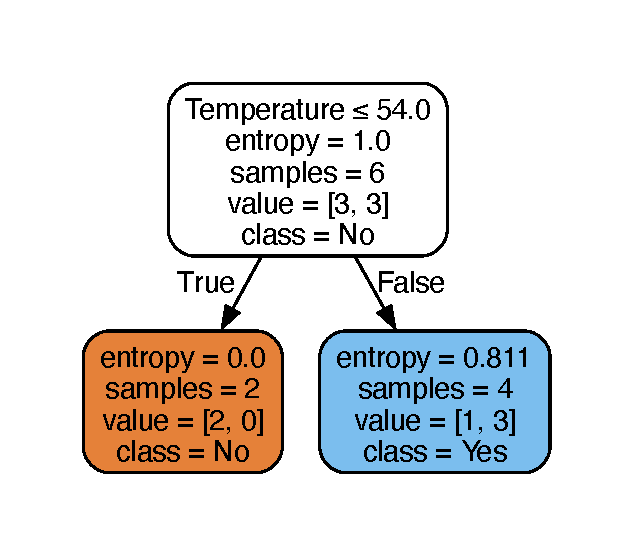
\includegraphics[scale=0.3]{../assets/decision-trees/figures/real-ip-1.pdf}
				\end{notebookbox}
				\end{frame}

				\begin{frame}{Finding splits}
					\begin{table}[]
						\begin{tabular}{@{}lrr@{}}
							\toprule
							\textbf{Day} & \textbf{Temperature} & \textbf{PlayTennis} \\ \midrule
							D1           & 40                   & No                  \\
							D2           & 48                   & No                  \\
							D3           & 60                   & Yes                 \\
							D4           & 72                   & Yes                 \\
							D5           & 80                   & Yes                 \\
							D6           & 90                   & No                  \\ \bottomrule
						\end{tabular}
					\end{table}
					\begin{notebookbox}{https://nipunbatra.github.io/ml-teaching/notebooks/decision-tree-real-input-discrete-output.html}
						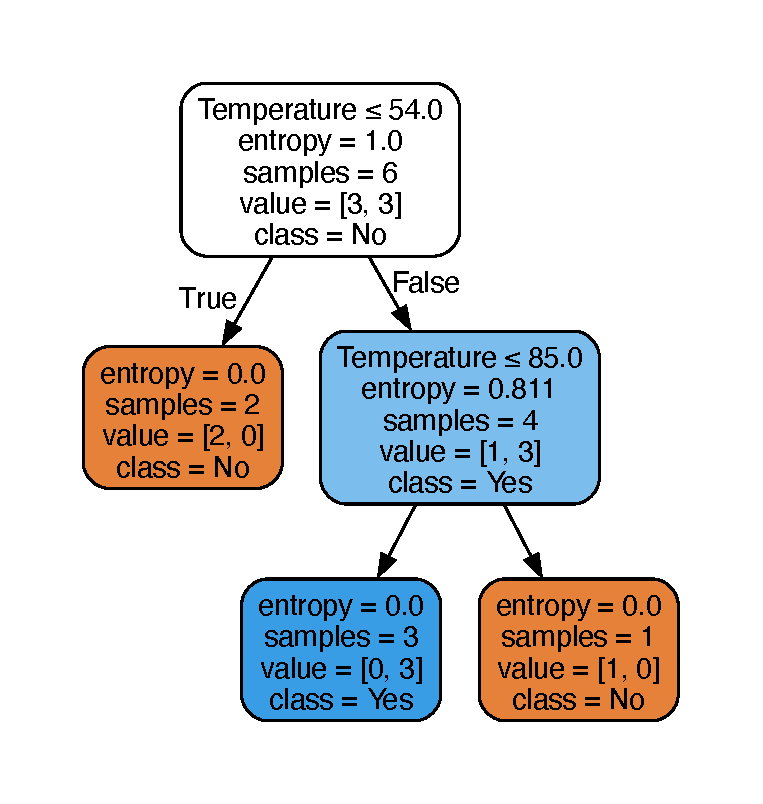
\includegraphics[scale=0.25]{../assets/decision-trees/figures/real-ip-2.pdf}
					\end{notebookbox}
					\end{frame}

\foreach \i in {1,...,9} {
\begin{frame}{Example (DT of depth \i)}
    \begin{figure}
		\centering
		\begin{notebookbox}{https://nipunbatra.github.io/ml-teaching/notebooks/decision-tree-real-input-discrete-output.html}
			\includegraphics{../assets/decision-trees/figures/dt-\i.pdf}
		  \end{notebookbox}
    
    \end{figure}
\end{frame}
}






\begin{frame}{Pop Quiz \stepcounter{popquiz}\#\thepopquiz}
\begin{tcolorbox}[colback=blue!5!white,colframe=blue!75!black,title=Quick Question!]
When finding splits for continuous features, how do we determine candidate split points?
\begin{enumerate}[A)]
\item Use all feature values as split points
\item Use midpoints between consecutive sorted feature values
\item Use random values within the feature range
\item Use only the minimum and maximum values
\end{enumerate}
\pause
\textbf{Answer: B) Use midpoints between consecutive sorted feature values} - This ensures we test all meaningful boundaries between different class regions.
\end{tcolorbox}
\end{frame}

\section{Real Input Real Output}

\begin{frame}{Example 1}
Let us consider the dataset given below
\begin{center}
	\begin{notebookbox}{https://nipunbatra.github.io/ml-teaching/notebooks/decision-tree-real-input-real-output.html}
		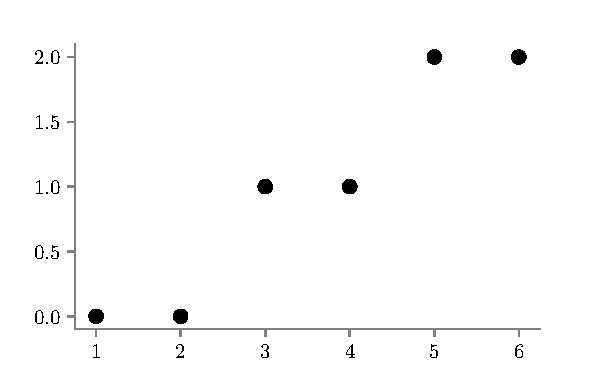
\includegraphics{../assets/decision-trees/figures/ri-ro-dataset.pdf}
	  \end{notebookbox}
\end{center}
\end{frame}

\begin{frame}{Example 1}
What would be the prediction for decision tree with depth 0?
\begin{center}
	\begin{notebookbox}{https://nipunbatra.github.io/ml-teaching/notebooks/decision-tree-real-input-real-output.html}
		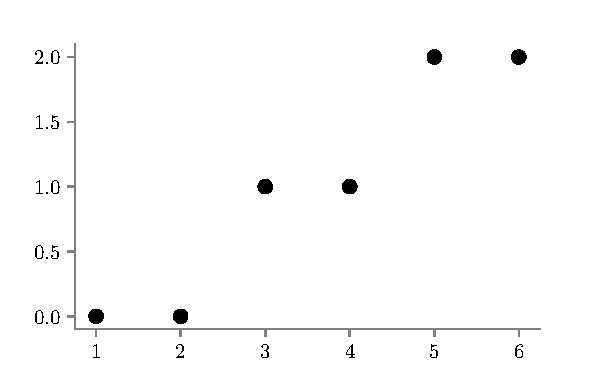
\includegraphics{../assets/decision-trees/figures/ri-ro-dataset.pdf}
	  \end{notebookbox}
\end{center}
\end{frame}

\begin{frame}{Example 1}
Prediction for decision tree with depth 0.\\
Horizontal dashed line shows the predicted $Y$ value. It is the average of $Y$ values of all datapoints.\\
\begin{center}
	\begin{notebookbox}{https://nipunbatra.github.io/ml-teaching/notebooks/decision-tree-real-input-real-output.html}
		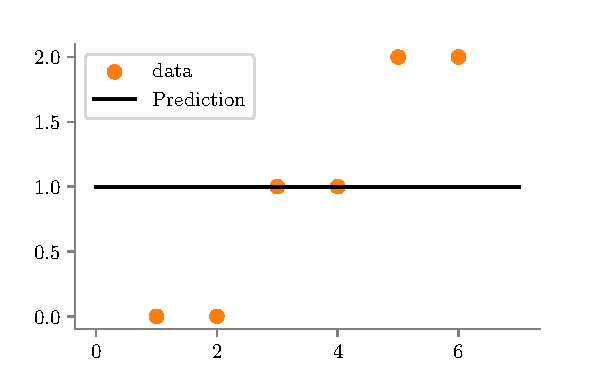
\includegraphics{../assets/decision-trees/figures/ri-ro-depth-0.pdf}	
	  \end{notebookbox}
\end{center}
\end{frame}


\begin{frame}{Example 1}
What would be the decision tree with depth 1?
\begin{center}
	\begin{notebookbox}{https://nipunbatra.github.io/ml-teaching/notebooks/decision-tree-real-input-real-output.html}
		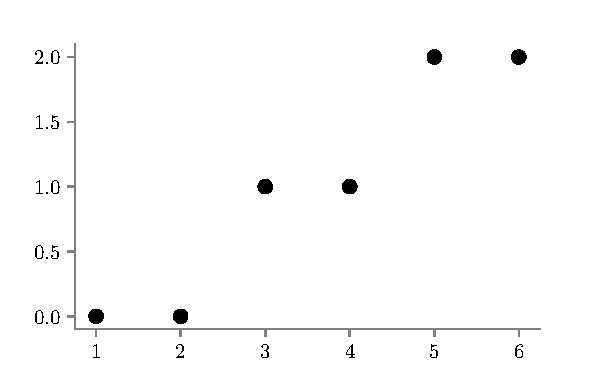
\includegraphics{../assets/decision-trees/figures/ri-ro-dataset.pdf}
	  \end{notebookbox}
\end{center}
\end{frame}

\begin{frame}{Example 1}
Decision tree with depth 1
\begin{center}
	\begin{notebookbox}{https://nipunbatra.github.io/ml-teaching/notebooks/decision-tree-real-input-real-output.html}
		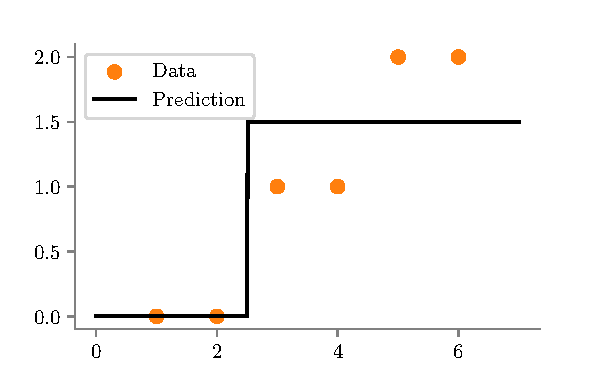
\includegraphics{../assets/decision-trees/figures/ri-ro-depth-1.pdf}
	\end{notebookbox}	
\end{center}
\end{frame}

\begin{frame}{Example 1}
The Decision Boundary
\begin{center}
	\begin{notebookbox}{https://nipunbatra.github.io/ml-teaching/notebooks/decision-tree-real-input-real-output.html}
		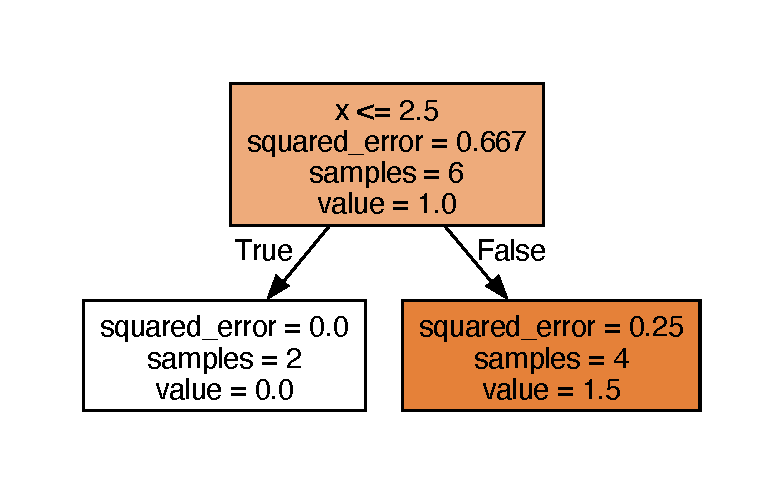
\includegraphics[scale=0.6]{../assets/decision-trees/figures/ri-ro-depth-1-sklearn.pdf}
	\end{notebookbox}
\end{center}
\end{frame}


\begin{frame}{Example 1}
What would be the decision tree with depth 2	?
\begin{center}
	\begin{notebookbox}{https://nipunbatra.github.io/ml-teaching/notebooks/decision-tree-real-input-real-output.html}
		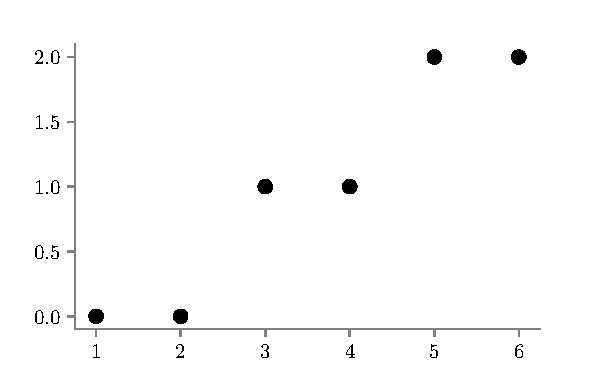
\includegraphics{../assets/decision-trees/figures/ri-ro-dataset.pdf}
	  \end{notebookbox}
\end{center}
\end{frame}

\begin{frame}{Example 1}
	Decision tree with depth 2
	\begin{center}
		\begin{notebookbox}{https://nipunbatra.github.io/ml-teaching/notebooks/decision-tree-real-input-real-output.html}
			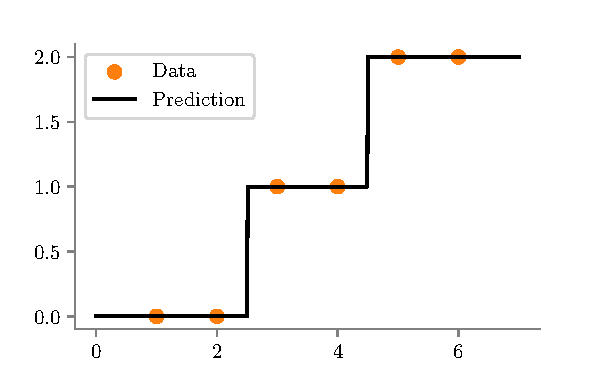
\includegraphics{../assets/decision-trees/figures/ri-ro-depth-2.pdf}
		\end{notebookbox}
	\end{center}
	\end{frame}
	
	\begin{frame}{Example 1}
	The Decision Boundary
	\begin{center}
		\begin{notebookbox}{https://nipunbatra.github.io/ml-teaching/notebooks/decision-tree-real-input-real-output.html}
			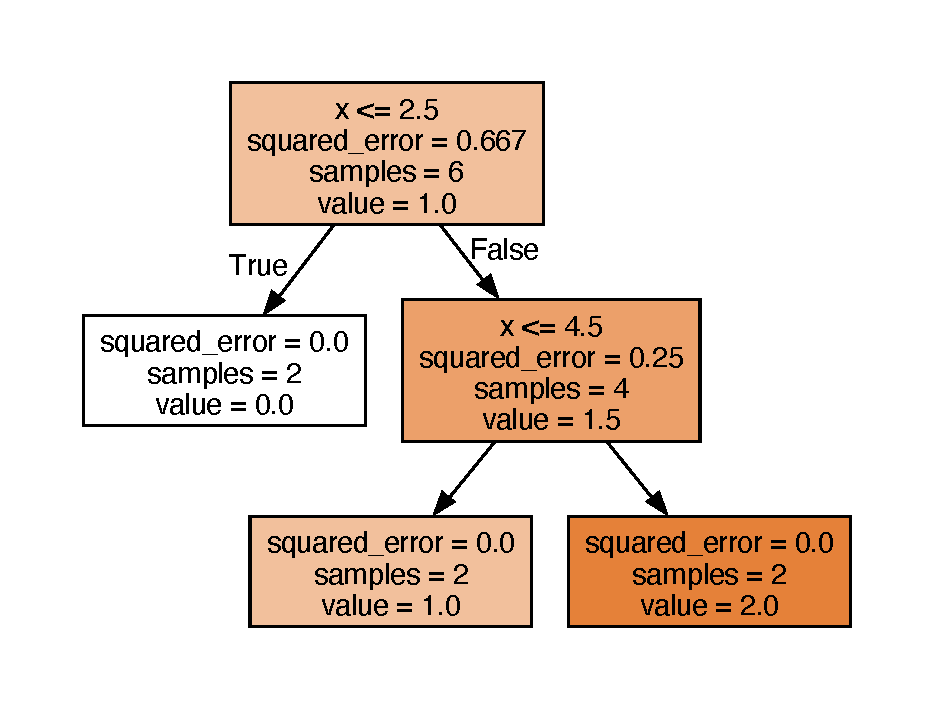
\includegraphics[scale=0.6]{../assets/decision-trees/figures/ri-ro-depth-2-sklearn.pdf}
		\end{notebookbox}
	\end{center}
	\end{frame}
	

\begin{frame}{Objective Function for Regression Trees}
\only<1-4>{
Feature is denoted by $X$ and target by $Y$.\\
Let the split be at $X = s$.\\
Define regions: $R_1 = \{x : x \leq s\}$ and $R_2 = \{x : x > s\}$.\\
\vspace{1cm}
}
\only<2-4>{
For each region, compute the mean prediction:\\
$c_1 = \frac{1}{|R_1|} \sum_{x_i \in R_1} y_i$ \\
$c_2 = \frac{1}{|R_2|} \sum_{x_i \in R_2} y_i$ \\
}
\only<3-4>{
The loss function is:\\
$$\text{Loss}(s) = \sum_{x_i \in R_1} (y_i - c_1)^2 + \sum_{x_i \in R_2} (y_i - c_2)^2$$
\vspace{1cm}
}
\only<4>{
Our objective is to find the optimal split:\\
$$s^* = \argmin_{s} \left[ \sum_{x_i \in R_1(s)} (y_i - c_1(s))^2 + \sum_{x_i \in R_2(s)} (y_i - c_2(s))^2 \right]$$
}
\end{frame}

\begin{frame}{Algorithm: Finding the Optimal Split}
\begin{enumerate}
\item<1-> Sort all data points $(x_i, y_i)$ in increasing order of $x_i$.
\item<2-> Evaluate the loss function for all candidate splits:
\vspace{0.25cm}
\begin{center}
$s = \frac{x_i + x_{i+1}}{2}$ for $i = 1, 2, \ldots, n-1$
\end{center}
\vspace{0.25cm}
\item<2-> Select the split $s^*$ that minimizes the loss function.
\end{enumerate} 
\end{frame}


\begin{frame}{A Question!}
Draw a regression tree for Y = sin(X), $0 \leq X \leq 2\pi$ 
\end{frame}

\begin{frame}{A Question!}
Dataset of Y = sin(X), $0 \leq X \leq 7$ with 10,000 points 
\begin{center}
	\begin{notebookbox}{https://nipunbatra.github.io/ml-teaching/notebooks/decision-tree-real-input-real-output.html}
		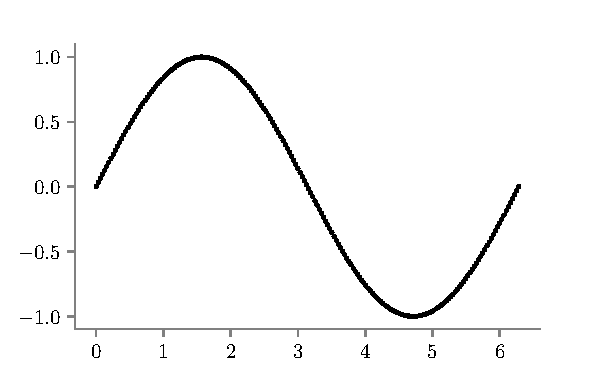
\includegraphics{../assets/decision-trees/figures/sine-dataset.pdf}
	  \end{notebookbox}
\end{center}
\end{frame}

\begin{frame}{A Question!}
Regression tree of depth 1
\begin{center}
	\begin{notebookbox}{https://nipunbatra.github.io/ml-teaching/notebooks/decision-tree-real-input-real-output.html}
		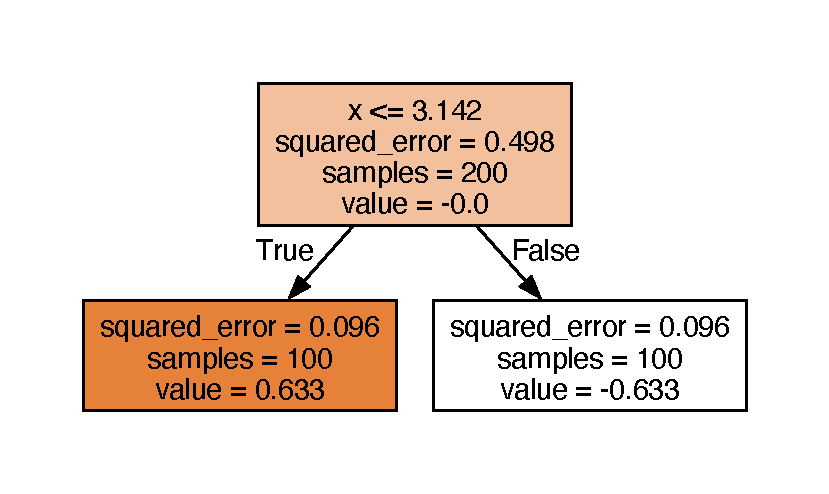
\includegraphics[scale=0.6]{../assets/decision-trees/figures/sine-depth-1-sklearn.pdf}
	  \end{notebookbox}
\end{center}
\end{frame}

\begin{frame}{A Question!}
Decision Boundary
\begin{center}
	\begin{notebookbox}{https://nipunbatra.github.io/ml-teaching/notebooks/decision-tree-real-input-real-output.html}
		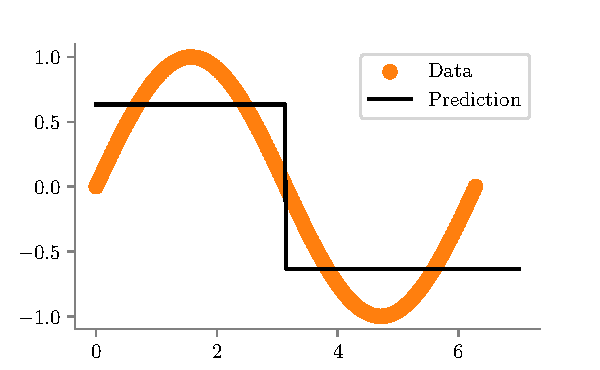
\includegraphics{../assets/decision-trees/figures/sine-depth-1.pdf}
	  \end{notebookbox}
\end{center}
\end{frame}

\begin{frame}{A Question!}
Regression tree with no depth limit is too big to fit in a slide. \\
It has of depth 4. The decision boundaries are in figure below.\\
\begin{center}
	\begin{notebookbox}{https://nipunbatra.github.io/ml-teaching/notebooks/decision-tree-real-input-real-output.html}
		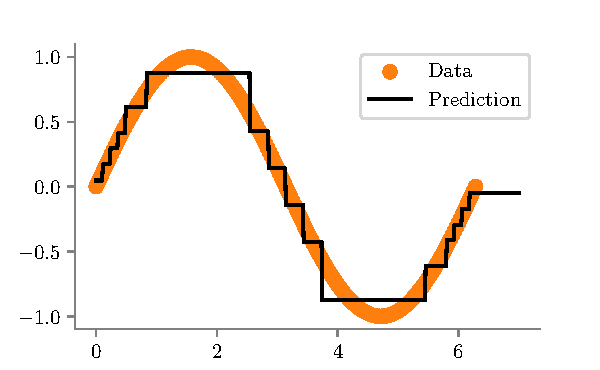
\includegraphics{../assets/decision-trees/figures/sine-depth-4.pdf}
	  \end{notebookbox}
\end{center}
\end{frame}

\begin{frame}{Pop Quiz \stepcounter{popquiz}\#\thepopquiz}
\begin{tcolorbox}[colback=blue!5!white,colframe=blue!75!black,title=Quick Question!]
What is the prediction function for a regression tree leaf node?
\begin{enumerate}[A)]
\item The median of target values in that region
\item The mode of target values in that region  
\item The mean of target values in that region
\item A linear function of the features
\end{enumerate}
\pause
\textbf{Answer: C) The mean of target values in that region} - Each leaf predicts the average target value of training samples that reach that leaf.
\end{tcolorbox}
\end{frame}

\section{Pruning and Overfitting}

\begin{frame}{The Problem: Overfitting in Decision Trees}
\begin{itemize}[<+->]
\item \textbf{Unpruned trees}: Can grow very deep and complex
\item \textbf{Perfect training accuracy}: Each leaf contains single training example
\item \textbf{But}: Poor generalization to new data
\item \textbf{Symptoms}:
    \begin{itemize}
    \item High training accuracy, low test accuracy
    \item Very deep trees with many leaves
    \item Rules that are too specific to training data
    \end{itemize}
\item \textbf{Solution}: Pruning to control model complexity
\end{itemize}
\end{frame}

\begin{frame}{Pre-pruning (Early Stopping)}
\textbf{Stop growing tree before it becomes too complex}:
\begin{itemize}[<+->]
\item \textbf{Maximum depth}: Limit tree depth (e.g., max\_depth = 5)
\item \textbf{Minimum samples per split}: Don't split if node has < N samples
\item \textbf{Minimum samples per leaf}: Ensure each leaf has $\geq$ M samples
\item \textbf{Maximum features}: Consider only subset of features at each split
\item \textbf{Minimum impurity decrease}: Only split if improvement > threshold
\end{itemize}

\textbf{Advantages}: Simple, computationally efficient \\
\textbf{Disadvantages}: May stop too early, miss good splits later
\end{frame}

\begin{frame}{Post-pruning (Tree Simplification)}
\textbf{Grow full tree, then remove unnecessary branches}:
\begin{itemize}[<+->]
\item \textbf{Algorithm}:
    \begin{enumerate}
    \item Grow complete tree on training data
    \item Use validation set to evaluate subtree performance
    \item Remove branches that don't improve validation accuracy
    \item Repeat until no beneficial removals remain
    \end{enumerate}
\item \textbf{Cost Complexity Pruning}: Minimize $\text{Error} + \alpha \times \text{Tree Size}$
\item \textbf{Advantages}: More thorough, can recover from early stopping mistakes
\item \textbf{Disadvantages}: More computationally expensive
\end{itemize}
\end{frame}

\begin{frame}{Cost Complexity Pruning Algorithm}
\textbf{Systematic approach to find optimal tree size}:
\begin{itemize}[<+->]
\item \textbf{Cost function}: $R_\alpha(T) = R(T) + \alpha |T|$
    \begin{itemize}
    \item $R(T)$: Misclassification error on validation set
    \item $|T|$: Number of terminal nodes (tree size)
    \item $\alpha$: Complexity parameter (penalty for larger trees)
    \end{itemize}
\item \textbf{Process}:
    \begin{enumerate}
    \item Start with full tree ($\alpha = 0$)
    \item Gradually increase $\alpha$
    \item At each $\alpha$, prune branches that increase cost
    \item Select $\alpha$ with best cross-validation performance
    \end{enumerate}
\end{itemize}
\end{frame}

\begin{frame}{Bias-Variance Trade-off in Trees}
\begin{itemize}[<+->]
\item \textbf{Unpruned trees}:
    \begin{itemize}
    \item Low bias (can fit complex patterns)
    \item High variance (sensitive to training data changes)
    \item Prone to overfitting
    \end{itemize}
\item \textbf{Heavily pruned trees}:
    \begin{itemize}
    \item High bias (may miss important patterns)
    \item Low variance (more stable predictions)
    \item Risk of underfitting
    \end{itemize}
\item \textbf{Optimal pruning}: Balances bias and variance
\item \textbf{Cross-validation}: Essential for finding this balance
\end{itemize}
\end{frame}

\begin{frame}{Practical Pruning Guidelines}
\begin{itemize}[<+->]
\item \textbf{Start simple}: Begin with restrictive pre-pruning parameters
\item \textbf{Cross-validation}: Always use CV to select pruning parameters
\item \textbf{Validation curves}: Plot training/validation error vs. tree complexity
\item \textbf{Common parameters} (sklearn):
    \begin{itemize}
    \item \texttt{max\_depth}: Start with 3-10
    \item \texttt{min\_samples\_split}: Try 10-100
    \item \texttt{min\_samples\_leaf}: Try 5-50
    \item \texttt{ccp\_alpha}: Use for cost complexity pruning
    \end{itemize}
\item \textbf{Domain knowledge}: Consider interpretability requirements
\end{itemize}
\end{frame}

\section{Summary and Key Takeaways}

\begin{frame}{Summary}
\begin{itemize}
	\item Interpretability an important goal
\item Decision trees: well known interpretable models
\item  Learning optimal tree is hard
\item  Greedy approach:
\item  Recursively split to maximize “performance gain”
\item  Issues:
\begin{itemize}
	\item Can overfit easily!
	\item  Empirically not as powerful as other methods
\end{itemize}
\end{itemize}

\end{frame}


\begin{frame}

	\begin{figure}
		\centering
		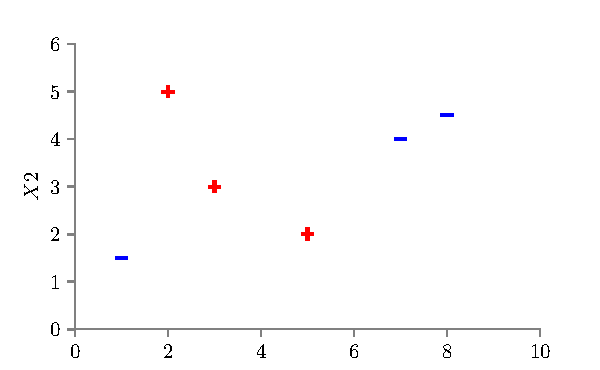
\includegraphics{../assets/decision-trees/figures/dt_weighted/fig1.pdf}
	\end{figure}
	
	
	\end{frame}
	
	
	\begin{frame}
	
	\begin{figure}
		\centering
		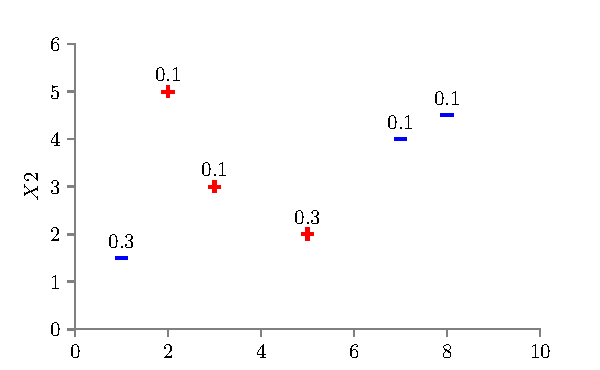
\includegraphics{../assets/decision-trees/figures/dt_weighted/fig2.pdf}
	\end{figure}
	
	
	\end{frame}
	
	
	\begin{frame}
	
	\begin{figure}
		\centering
		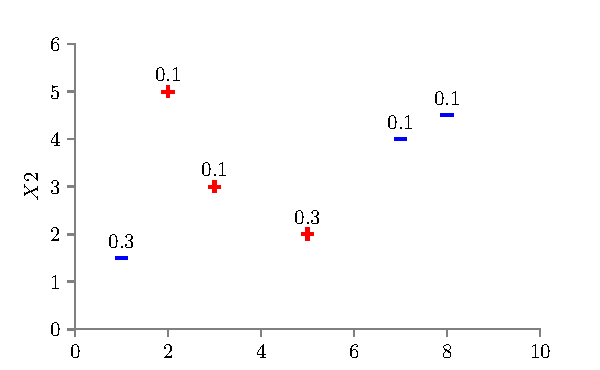
\includegraphics{../assets/decision-trees/figures/dt_weighted/fig2.pdf}
	\end{figure}
	
	$$\Entropy = -P(+) \log_2 P(+) - P(-) \log_2 P(-)$$
	
	$$P(+) = \frac{0.1 + 0.1 + 0.3}{1} = 0.5, \quad P(-) = \frac{0.3 + 0.1 + 0.1}{1} = 0.5$$
	
	$$\Entropy = E_s = -\frac{1}{2} \log_2 \frac{1}{2} - \frac{1}{2} \log_2 \frac{1}{2} = 1$$
	
	\end{frame}
	
	
	\begin{section}{Weighted Entropy}
	
	
	
	\begin{frame}
	
	\begin{figure}
		\centering
		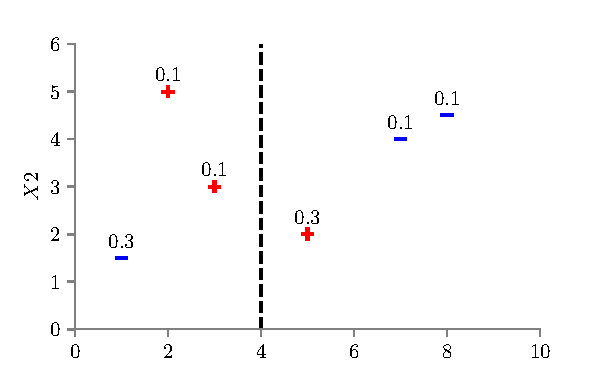
\includegraphics{../assets/decision-trees/figures/dt_weighted/fig3.pdf}
	\end{figure}
	
	
	Candidate Line: \(X1 = 4 (X1^*)\)
	
	
	\end{frame}
	
	
	\begin{frame}
	\begin{figure}
		\centering
		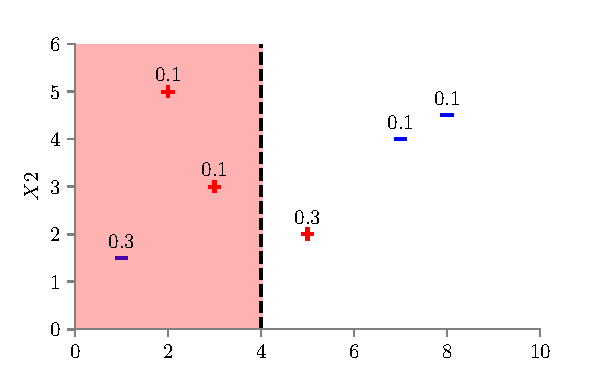
\includegraphics{../assets/decision-trees/figures/dt_weighted/fig4.pdf}
	\end{figure}
	
	Entropy of \(X1 \leq X1^*  = E_{S(X1 < X1^*)}\)
	
	$$P(+) = \frac{0.1 + 0.1}{0.1 + 0.1 + 0.3} = \frac{2}{5}$$
	
	$$P(-) = \frac{3}{5}$$
	
	
	\end{frame}
	
	
	\begin{frame}
	
	\begin{figure}
		\centering
		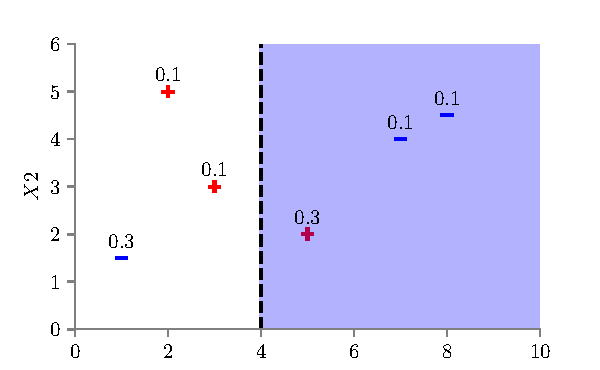
\includegraphics{../assets/decision-trees/figures/dt_weighted/fig5.pdf}
	\end{figure}
	Entropy of $X_1 > X_1^* = E_{S(X_1 > X_1^*)}$
	
	$$P(+) = \frac{3}{5}$$
	
	$$P(-) = \frac{2}{5}$$
	
	\end{frame}
	
	
	
	\begin{frame}
	
	\begin{figure}
		\centering
		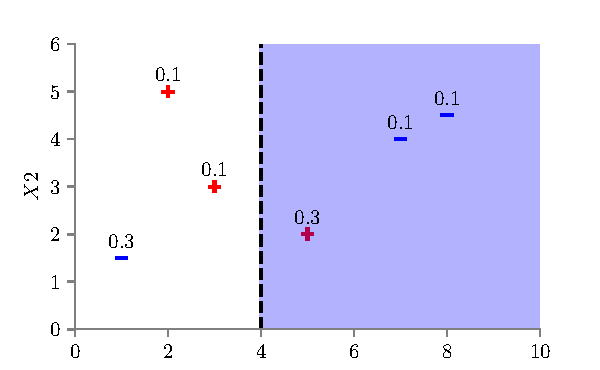
\includegraphics{../assets/decision-trees/figures/dt_weighted/fig5.pdf}
	\end{figure}
	
	$$\text{IG}(X_1 = X_1^*) = E_S - \frac{0.5}{1} \cdot E_{S(X_1 < X_1^*)} - \frac{0.5}{1} \cdot E_{S(X_1 > X_1^*)}$$
	
	\end{frame}

\end{section}
\end{document}
